% ============================================================
%  实验报告（第 2 周）— 王本熙 (25020007117)
%  编译方式: xelatex report2.tex (运行两遍以解析交叉引用)
% ============================================================
\documentclass[a4paper,11pt]{ctexart}

% ---------- 页面布局 ----------
\usepackage[
  top=2.5cm, bottom=2.5cm, left=2.5cm, right=2.5cm,
  headheight=15pt, headsep=0.5cm, footskip=0.8cm
]{geometry}

% ---------- 数学与表格 ----------
\usepackage{amsmath, amssymb}
\usepackage{booktabs}
\usepackage{array}
\usepackage{multirow}

% ---------- 图形与链接 ----------
\usepackage{graphicx}
\usepackage{subcaption}   % 子图支持
\usepackage[
  colorlinks=true, linkcolor=blue!70!black,
  citecolor=blue!70!black, urlcolor=teal!80!black
]{hyperref}
\usepackage{xcolor}

% ---------- 代码块 ----------
\usepackage{listings}
\definecolor{codebg}{RGB}{248,248,248}
\definecolor{codekw}{RGB}{0,0,180}
\definecolor{codecmt}{RGB}{0,128,0}
\definecolor{codestr}{RGB}{180,0,0}
\lstset{
  backgroundcolor=\color{codebg},
  basicstyle=\ttfamily\small,
  keywordstyle=\color{codekw}\bfseries,
  commentstyle=\color{codecmt},
  stringstyle=\color{codestr},
  numbers=left, numberstyle=\tiny\color{gray},
  frame=single, rulecolor=\color{gray!40},
  breaklines=true, showstringspaces=false,
  tabsize=2, columns=flexible,
  language=bash
}

% ---------- 页眉页脚 ----------
\usepackage{fancyhdr}
\pagestyle{fancy}
\fancyhf{}
\fancyhead[L]{\small 王本熙 \quad 25020007117}
\fancyhead[R]{\small 实验报告（第 2 周）}
\fancyfoot[C]{\thepage}
\renewcommand{\headrulewidth}{0.4pt}

% ---------- 章节标题样式 ----------
\usepackage{titlesec}
\definecolor{secblue}{RGB}{30,80,160}
\titleformat{\section}
  {\Large\bfseries\color{secblue}}{第\thesection\,章}{0.6em}{}
\titleformat{\subsection}
  {\large\bfseries\color{secblue!80!black}}{\thesubsection}{0.5em}{}
\titleformat{\subsubsection}
  {\normalsize\bfseries\color{secblue!60!black}}{\thesubsubsection}{0.5em}{}

% ---------- 超链接元信息 ----------
\hypersetup{
  pdftitle={系统开发工具基础实验报告（第 2 周）},
  pdfauthor={王本熙}
}

% ============================================================
\begin{document}

% ---------- 封面 ----------
\begin{titlepage}
  \centering
  \vspace*{2cm}
  {\Huge\bfseries\color{secblue} 实验报告\par}
  \vspace{0.5cm}
  {\Large 系统开发工具基础 \quad 第 2 周\par}
  \vspace{3cm}
  \begin{tabular}{rl}
    \Large 姓\quad 名\,:\, & \Large 王本熙 \\[0.8em]
    \Large 学\quad 号\,:\, & \Large 25020007117 \\[0.8em]
    \Large 日\quad 期\,:\, & \Large 2026 年 8 月 31 日 \\[0.8em]
    \Large 平\quad 台\,:\, & \Large Windows + WSL (Ubuntu) \\
  \end{tabular}
  \vfill
  \rule{10cm}{0.4pt}
  \vspace*{1cm}
\end{titlepage}

% ---------- 目录 ----------
\tableofcontents
\newpage

% ============================================================
\section{实验目的}

本实验旨在掌握以下内容：
\begin{itemize}
  \item 命令行环境下的进程与任务控制：前台/后台切换（\texttt{Ctrl-Z}、\texttt{bg}、\texttt{jobs}）；
  \item 信号机制：\texttt{trap} 捕获 \texttt{SIGTERM}/\texttt{SIGINT} 实现优雅退出（q05）；
  \item 语义重构与本地开发反馈：跳转定义、查找引用、符号重命名，
        配合 ruff 静态检查与 pytest 单元测试（q06）；
  \item 使用 pdb 调试器设断点、单步执行并观察变量，定位并最小修复归并排序缺陷（q07）；
  \item 性能分析驱动的优化流程：\texttt{time} 计时、\texttt{cProfile} 剖析定位热点、
        数据结构优化与加速比评估（q08）；
  \item 课后练习：命令行技巧、SSH 远程开发、Vim mode 配置，
        以及 rr / ASan / strace / perf 等调试与性能工具的扩展训练。
\end{itemize}

% ============================================================
\section{实验环境}

\begin{table}[htbp]
  \centering
  \caption{实验环境}\label{tab:env}
  \begin{tabular}{ll}
    \toprule
    项目 & 配置 \\
    \midrule
    操作系统 & Windows + WSL (Ubuntu) \\
    Shell & bash \\
    编辑器 & VS Code / Trae IDE / micro \\
    版本管理 & Git \\
    远程仓库 & GitHub \\
    \bottomrule
  \end{tabular}
\end{table}

% ============================================================
\section{q05：控制一个可清理的后台任务}

\subsection{题目要求}

主题：命令行环境——进程、信号与任务控制。将给定脚本保存为
\texttt{q05/worker.sh}，完成任务控制：
\begin{itemize}
  \item 赋予脚本执行权限，在前台启动，并把 stdout、stderr 分别写入
        \texttt{stdout.log}、\texttt{stderr.log}；
  \item 使用 \texttt{Ctrl-Z} 挂起任务，再用 \texttt{bg} 让它在后台继续；
        使用 \texttt{jobs} 确认状态；
  \item 使用 \texttt{jobs -p} 或等价方式取得 PID（不得手工抄写），
        发送 \texttt{SIGTERM} 并等待任务结束；
  \item 确认 \texttt{cleanup.log} 中出现 \texttt{CLEAN\_EXIT}，且任务已经退出；
        禁止使用 \texttt{kill -9}。
\end{itemize}

\subsection{实验步骤}

按题目给定的脚本内容写入 \texttt{work.sh}（初次操作时文件名误写为
\texttt{worker.sh} 与实际文件不一致，\texttt{chmod} 报错后统一改用
\texttt{work.sh}，不影响任务控制目标的完成）：

\begin{lstlisting}[language=bash]
#!/usr/bin/env bash
trap 'echo CLEAN_EXIT >> cleanup.log; exit 0' TERM INT
n=0
while true; do
  echo "$n"
  n=$((n+1))
  sleep 1
done
\end{lstlisting}

随后在 WSL (Ubuntu) 终端中依次执行：

\begin{lstlisting}[language=bash]
mkdir q05 && cd q05
touch work.sh
micro work.sh                      # 写入上述脚本
chmod +x work.sh                   # 赋予执行权限

./work.sh > stdout.log 2> stderr.log   # 前台启动, stdout/stderr 分别重定向
# Ctrl-Z 挂起 → [1]+ Stopped
bg                                 # 转入后台继续 → [1]+ Running
jobs                               # 确认后台运行状态

PID=$(jobs -p)                     # 取任务 PID(不手工抄写)
kill $PID                          # 默认发送 SIGTERM
jobs                               # 等待并确认 → [1]+ Done

cat cleanup.log                    # 验证 CLEAN_EXIT
cat stdout.log                     # 计数输出 0..17
cat stderr.log                     # 为空
\end{lstlisting}

\subsection{运行结果与截图}

图~\ref{fig:q05} 记录了完整的任务控制过程。

\begin{figure}[htbp]
  \centering
  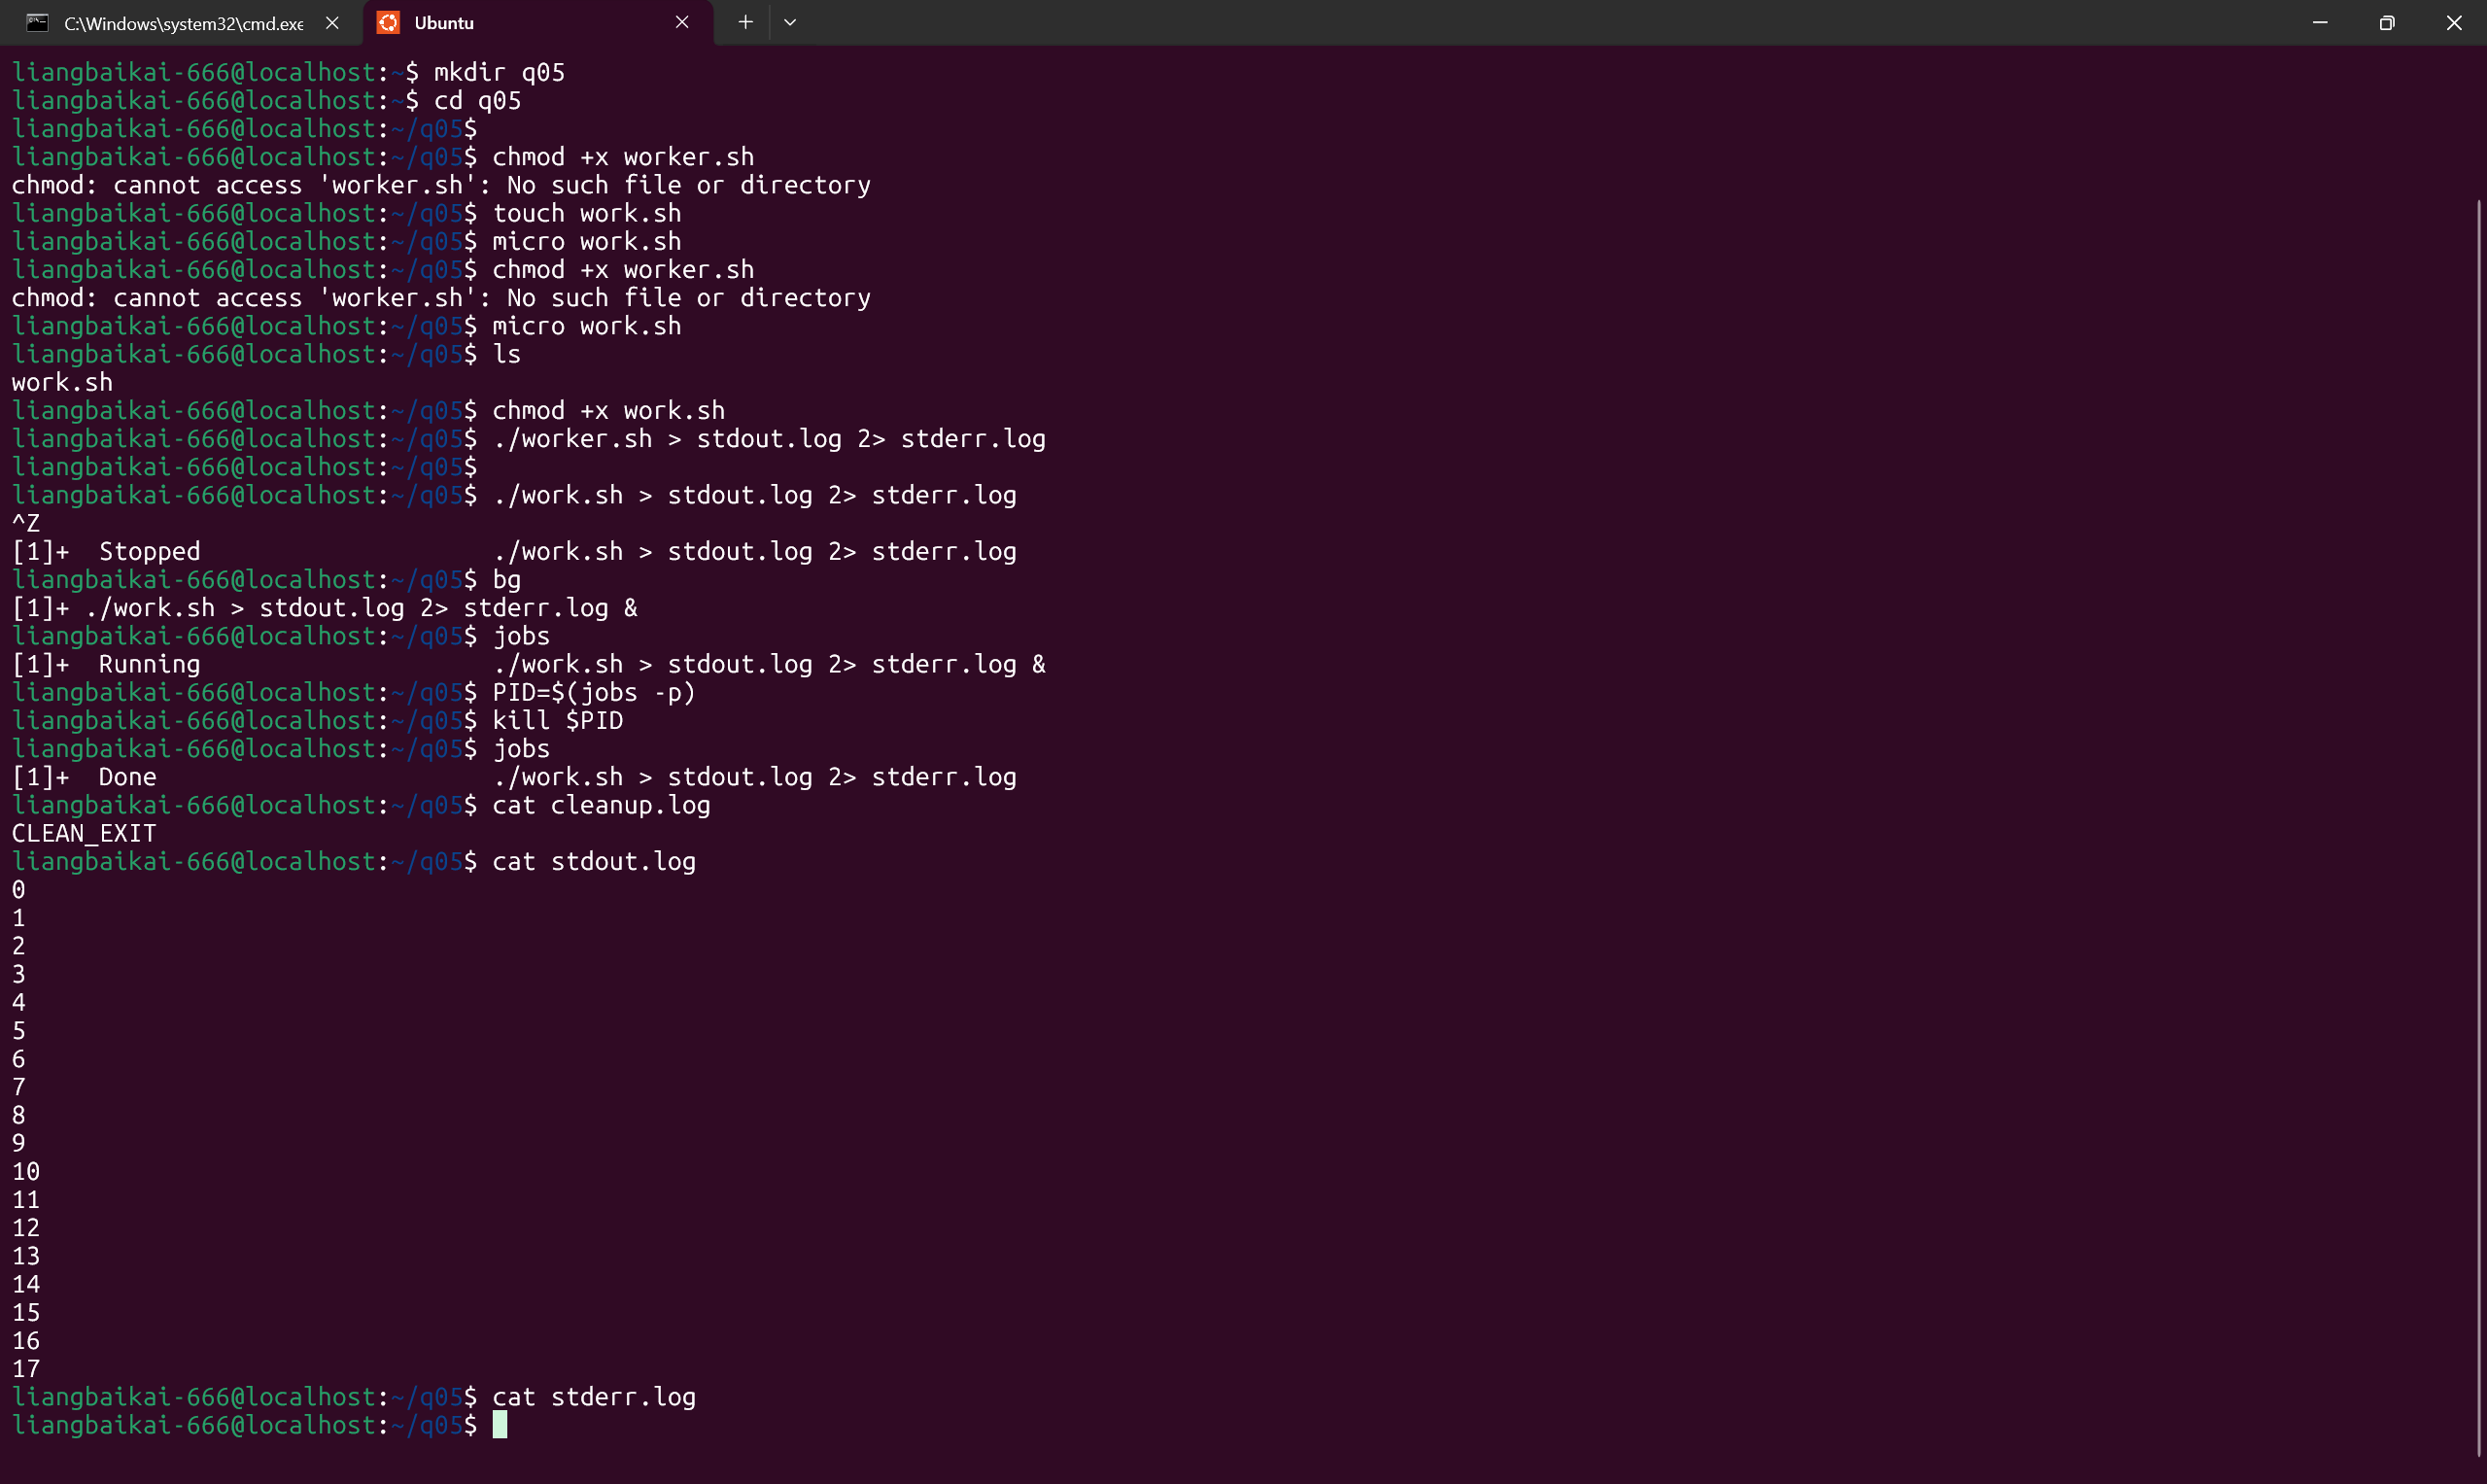
\includegraphics[width=0.98\textwidth]{q05-1.png}
  \caption{q05：前台启动、Ctrl-Z 挂起、bg 转后台、SIGTERM 优雅退出与日志验证}
  \label{fig:q05}
\end{figure}

\subsection{结果分析}

\begin{itemize}
  \item \textbf{任务状态切换}：\texttt{Ctrl-Z} 向前台进程发送 \texttt{SIGTSTP}，
        \texttt{jobs} 显示 \texttt{[1]+ Stopped}；\texttt{bg} 使任务在后台继续
        （等效于发送 \texttt{SIGCONT}），\texttt{jobs} 确认 \texttt{[1]+ Running}；
  \item \textbf{PID 获取与信号发送}：\texttt{PID=\$(jobs -p)} 从作业表取 PID，
        避免手工抄写出错；\texttt{kill \$PID} 默认发送 \texttt{SIGTERM}（信号 15），
        全程未使用 \texttt{kill -9}；
  \item \textbf{优雅退出}：脚本通过 \texttt{trap} 捕获 \texttt{TERM}/\texttt{INT} 信号，
        收到 \texttt{SIGTERM} 后先向 \texttt{cleanup.log} 追加 \texttt{CLEAN\_EXIT}
        再以退出码 0 结束；\texttt{jobs} 显示 \texttt{Done}，\texttt{cleanup.log}
        中确认出现 \texttt{CLEAN\_EXIT}；
  \item \textbf{重定向验证}：\texttt{stdout.log} 记录计数 0--17 共 18 行，
        表明任务前台与后台合计运行约 18 秒；\texttt{stderr.log} 为空，
        说明正常路径下脚本无错误输出。另注：首次误运行
        \texttt{./worker.sh} 的报错信息曾写入 \texttt{stderr.log}，
        被正式运行的 \texttt{2>} 截断覆盖，故最终为空。
\end{itemize}

% ============================================================
\section{q06：语义重构与本地开发反馈}

\subsection{题目要求}

主题：开发环境与工具。在 q06 中按照给定代码创建三个 Python 文件，
并使用编辑器语言服务器完成一次语义重构：
\begin{itemize}
  \item 在已配置好 Python、pytest 和 ruff 的课程环境中打开 q06，
        并启用 Python 语言服务器；
  \item 分别演示跳转到定义和查找引用；
  \item 使用``重命名符号''把 \texttt{total\_price} 改为 \texttt{calculate\_total}，
        保证定义和所有代码引用同步改变；
  \item 在 \texttt{app.py} 中临时加入未使用的 \texttt{import os}，
        用 ruff 发现并删除；最后运行 ruff 和 pytest 并保证通过。
\end{itemize}

\subsection{实验步骤}

按题目给定内容创建三个文件：

\begin{lstlisting}[language=Python]
# math_utils.py
def total_price(price: float, count: int) -> float:
    return price * count

# app.py
from math_utils import total_price
print(total_price(12.5, 4))

# test_math_utils.py
from math_utils import total_price

def test_total_price():
    assert total_price(12.5, 4) == 50.0
\end{lstlisting}

随后完成语义重构与质量检查（在 WSL 终端中以
\texttt{grep}/\texttt{sed} 完成``查找引用''与``重命名符号''的等效操作）：

\begin{lstlisting}[language=bash]
mkdir -p q06 && cd q06
micro math_utils.py app.py test_math_utils.py   # 写入三个给定文件

# 查找引用(等效 LSP "Find References")
grep -rn "total_price" *.py

# 语义重命名: 定义与全部引用同步改变(等效 LSP "Rename Symbol")
sed -i 's/total_price/calculate_total/g' *.py

# 再次查找, 验证重命名同步、无遗漏
grep -rn "calculate_total" *.py

# ruff 本地质量反馈环
micro app.py                 # 临时加入未使用的 import os
ruff check app.py            # F401 `os` imported but unused (app.py:1:8)
ruff check --fix app.py      # Found 2 errors (2 fixed, 0 remaining)
ruff check app.py            # All checks passed!

# pytest 回归
cd ~
pytest q06/test_math_utils.py    # 1 passed in 0.01s
\end{lstlisting}

\subsection{运行结果与截图}

图~\ref{fig:q06} 展示了从创建文件、语义重命名到 ruff/pytest 全部通过的过程。

\begin{figure}[htbp]
  \centering
  \begin{subfigure}[b]{0.98\textwidth}
    \centering
    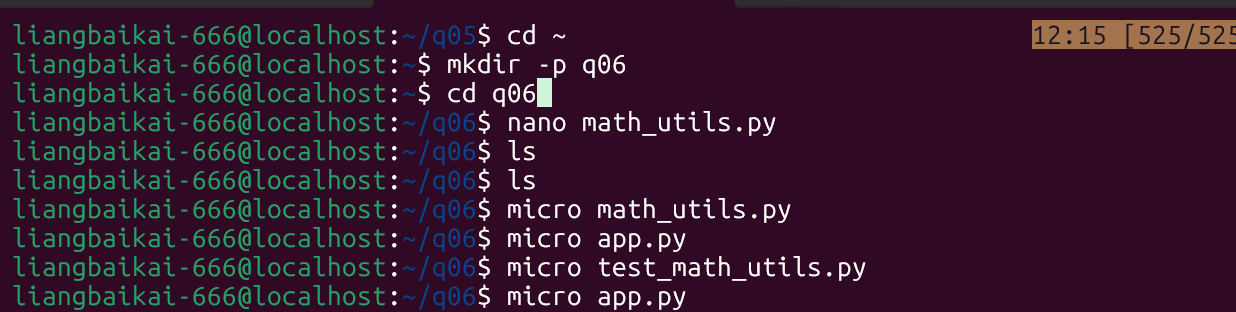
\includegraphics[width=\linewidth]{q06-1.png}
    \caption{创建 \texttt{math\_utils.py}、\texttt{app.py}、\texttt{test\_math\_utils.py}}
  \end{subfigure}

  \vspace{0.5em}
  \begin{subfigure}[b]{0.98\textwidth}
    \centering
    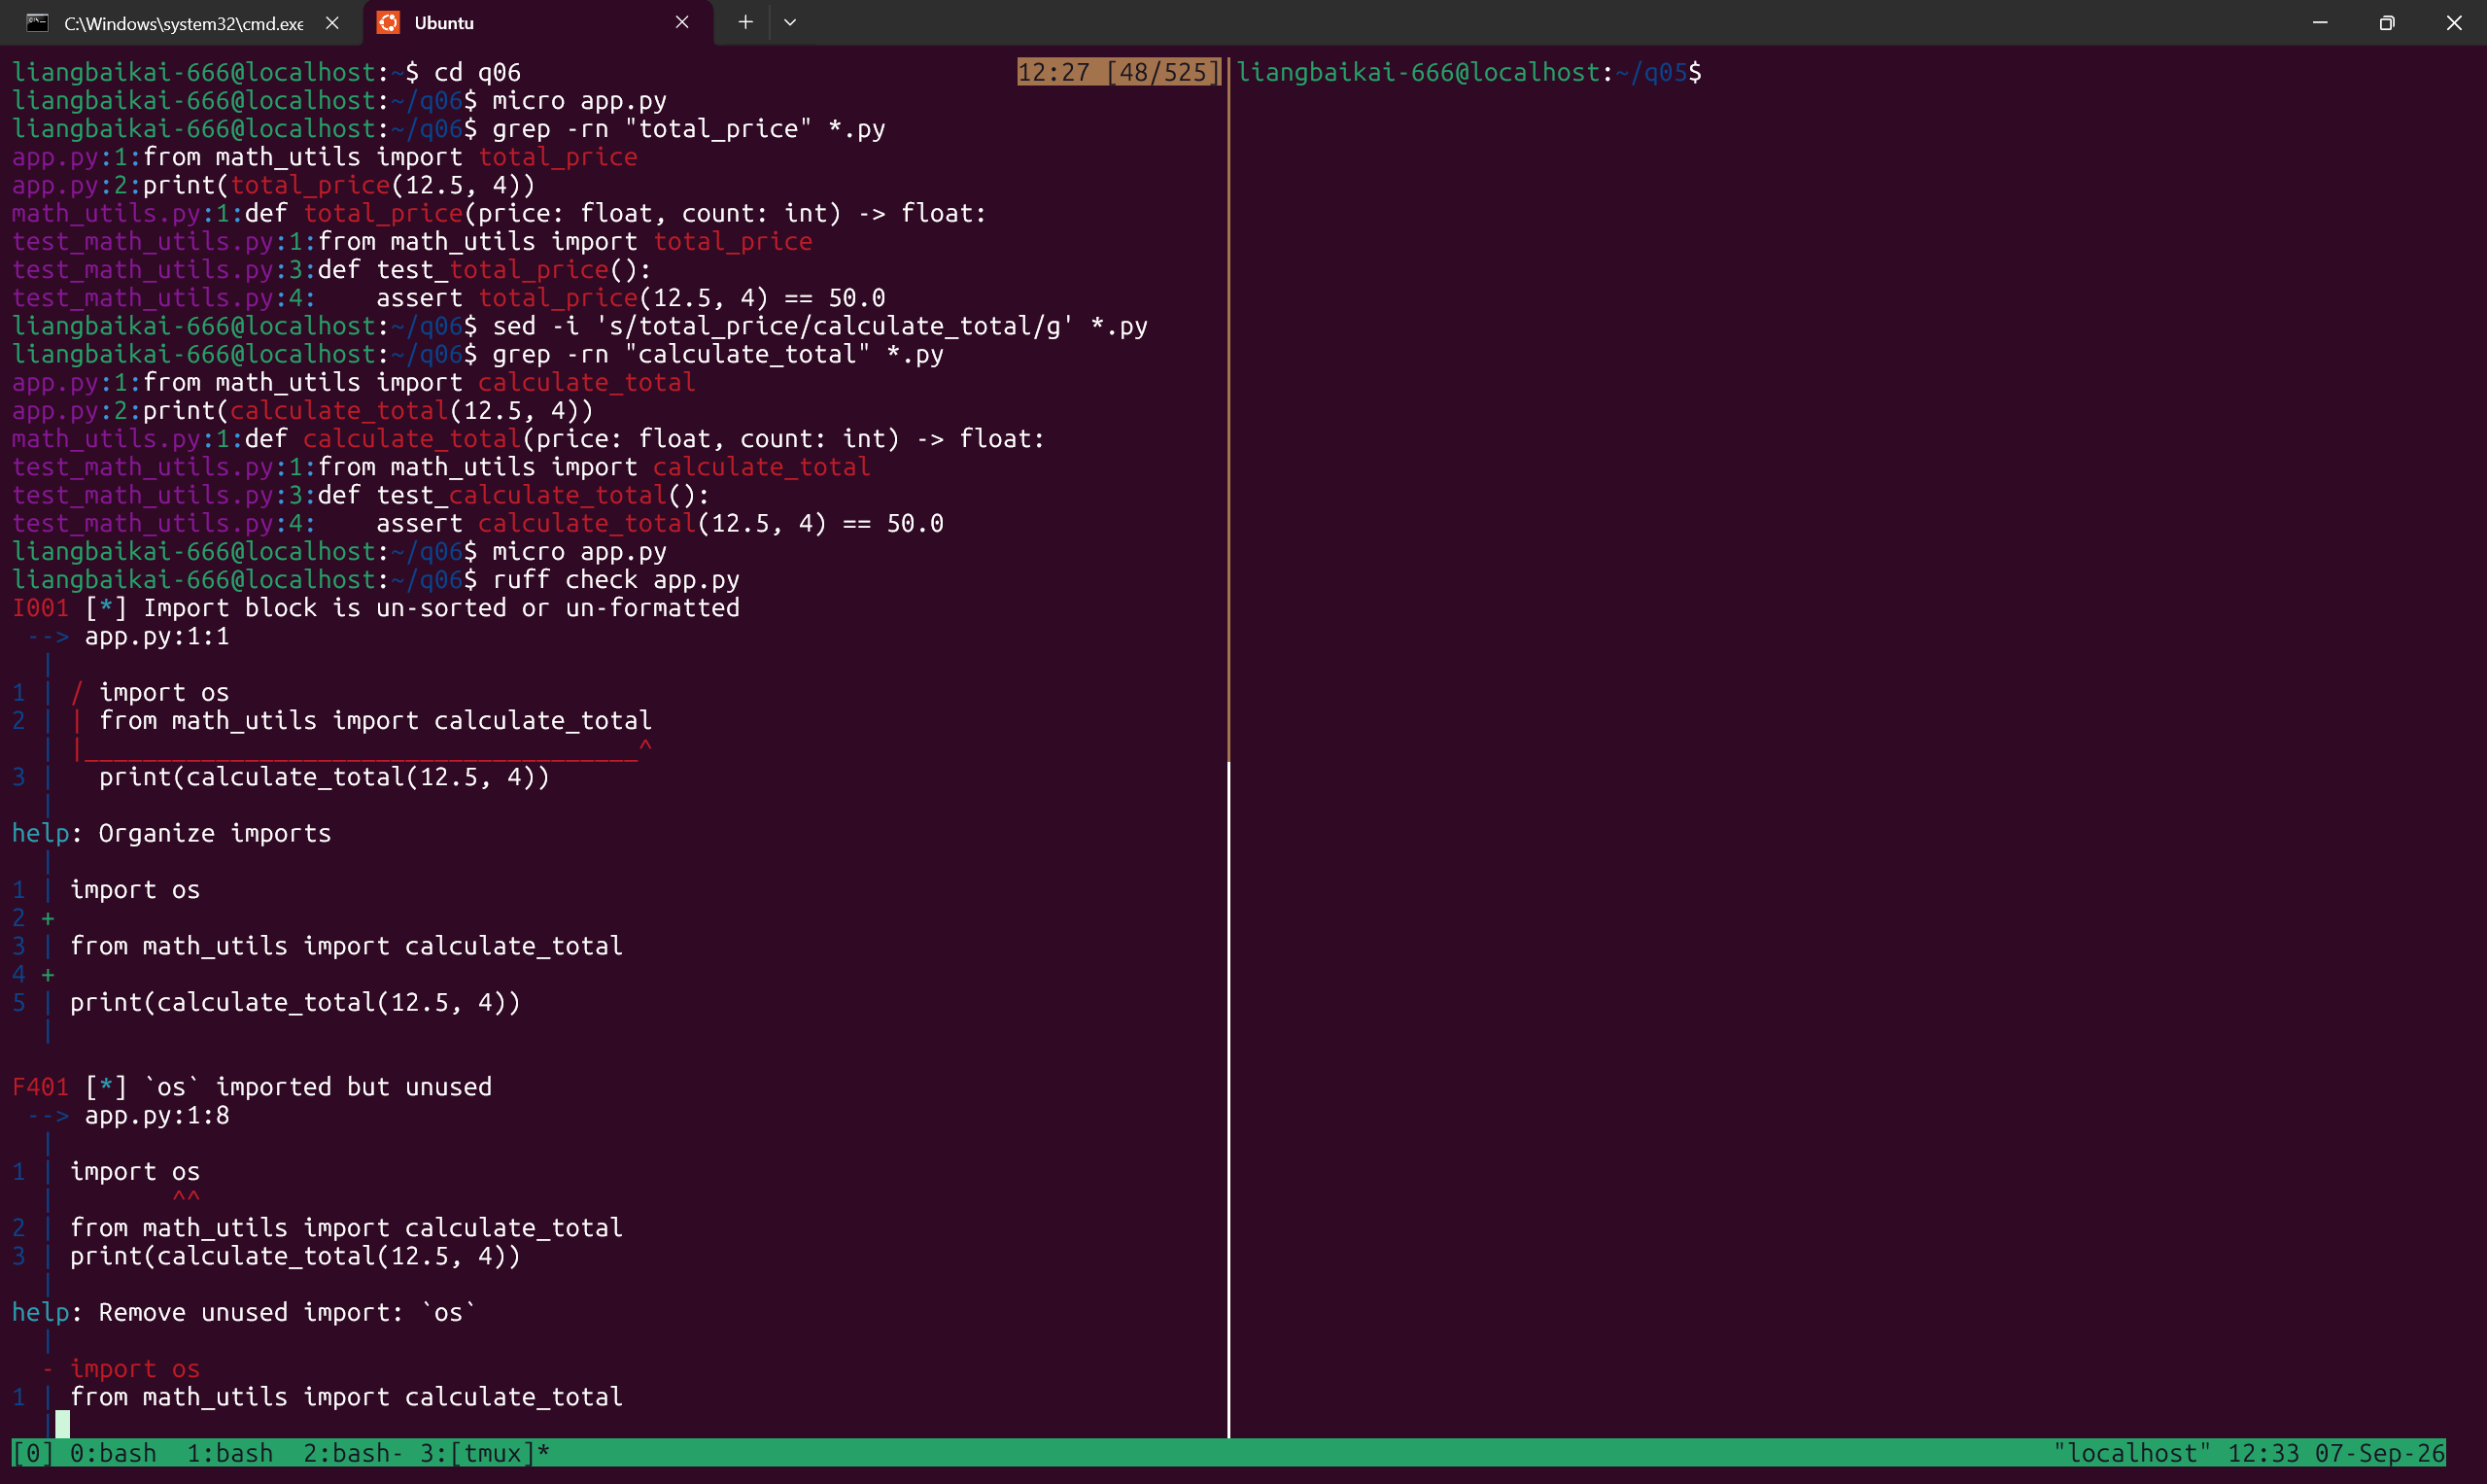
\includegraphics[width=\linewidth]{q06-2.png}
    \caption{\texttt{sed} 批量重命名标识符 + \texttt{ruff check} 发现 F401 未使用导入}
  \end{subfigure}

  \vspace{0.5em}
  \begin{subfigure}[b]{0.98\textwidth}
    \centering
    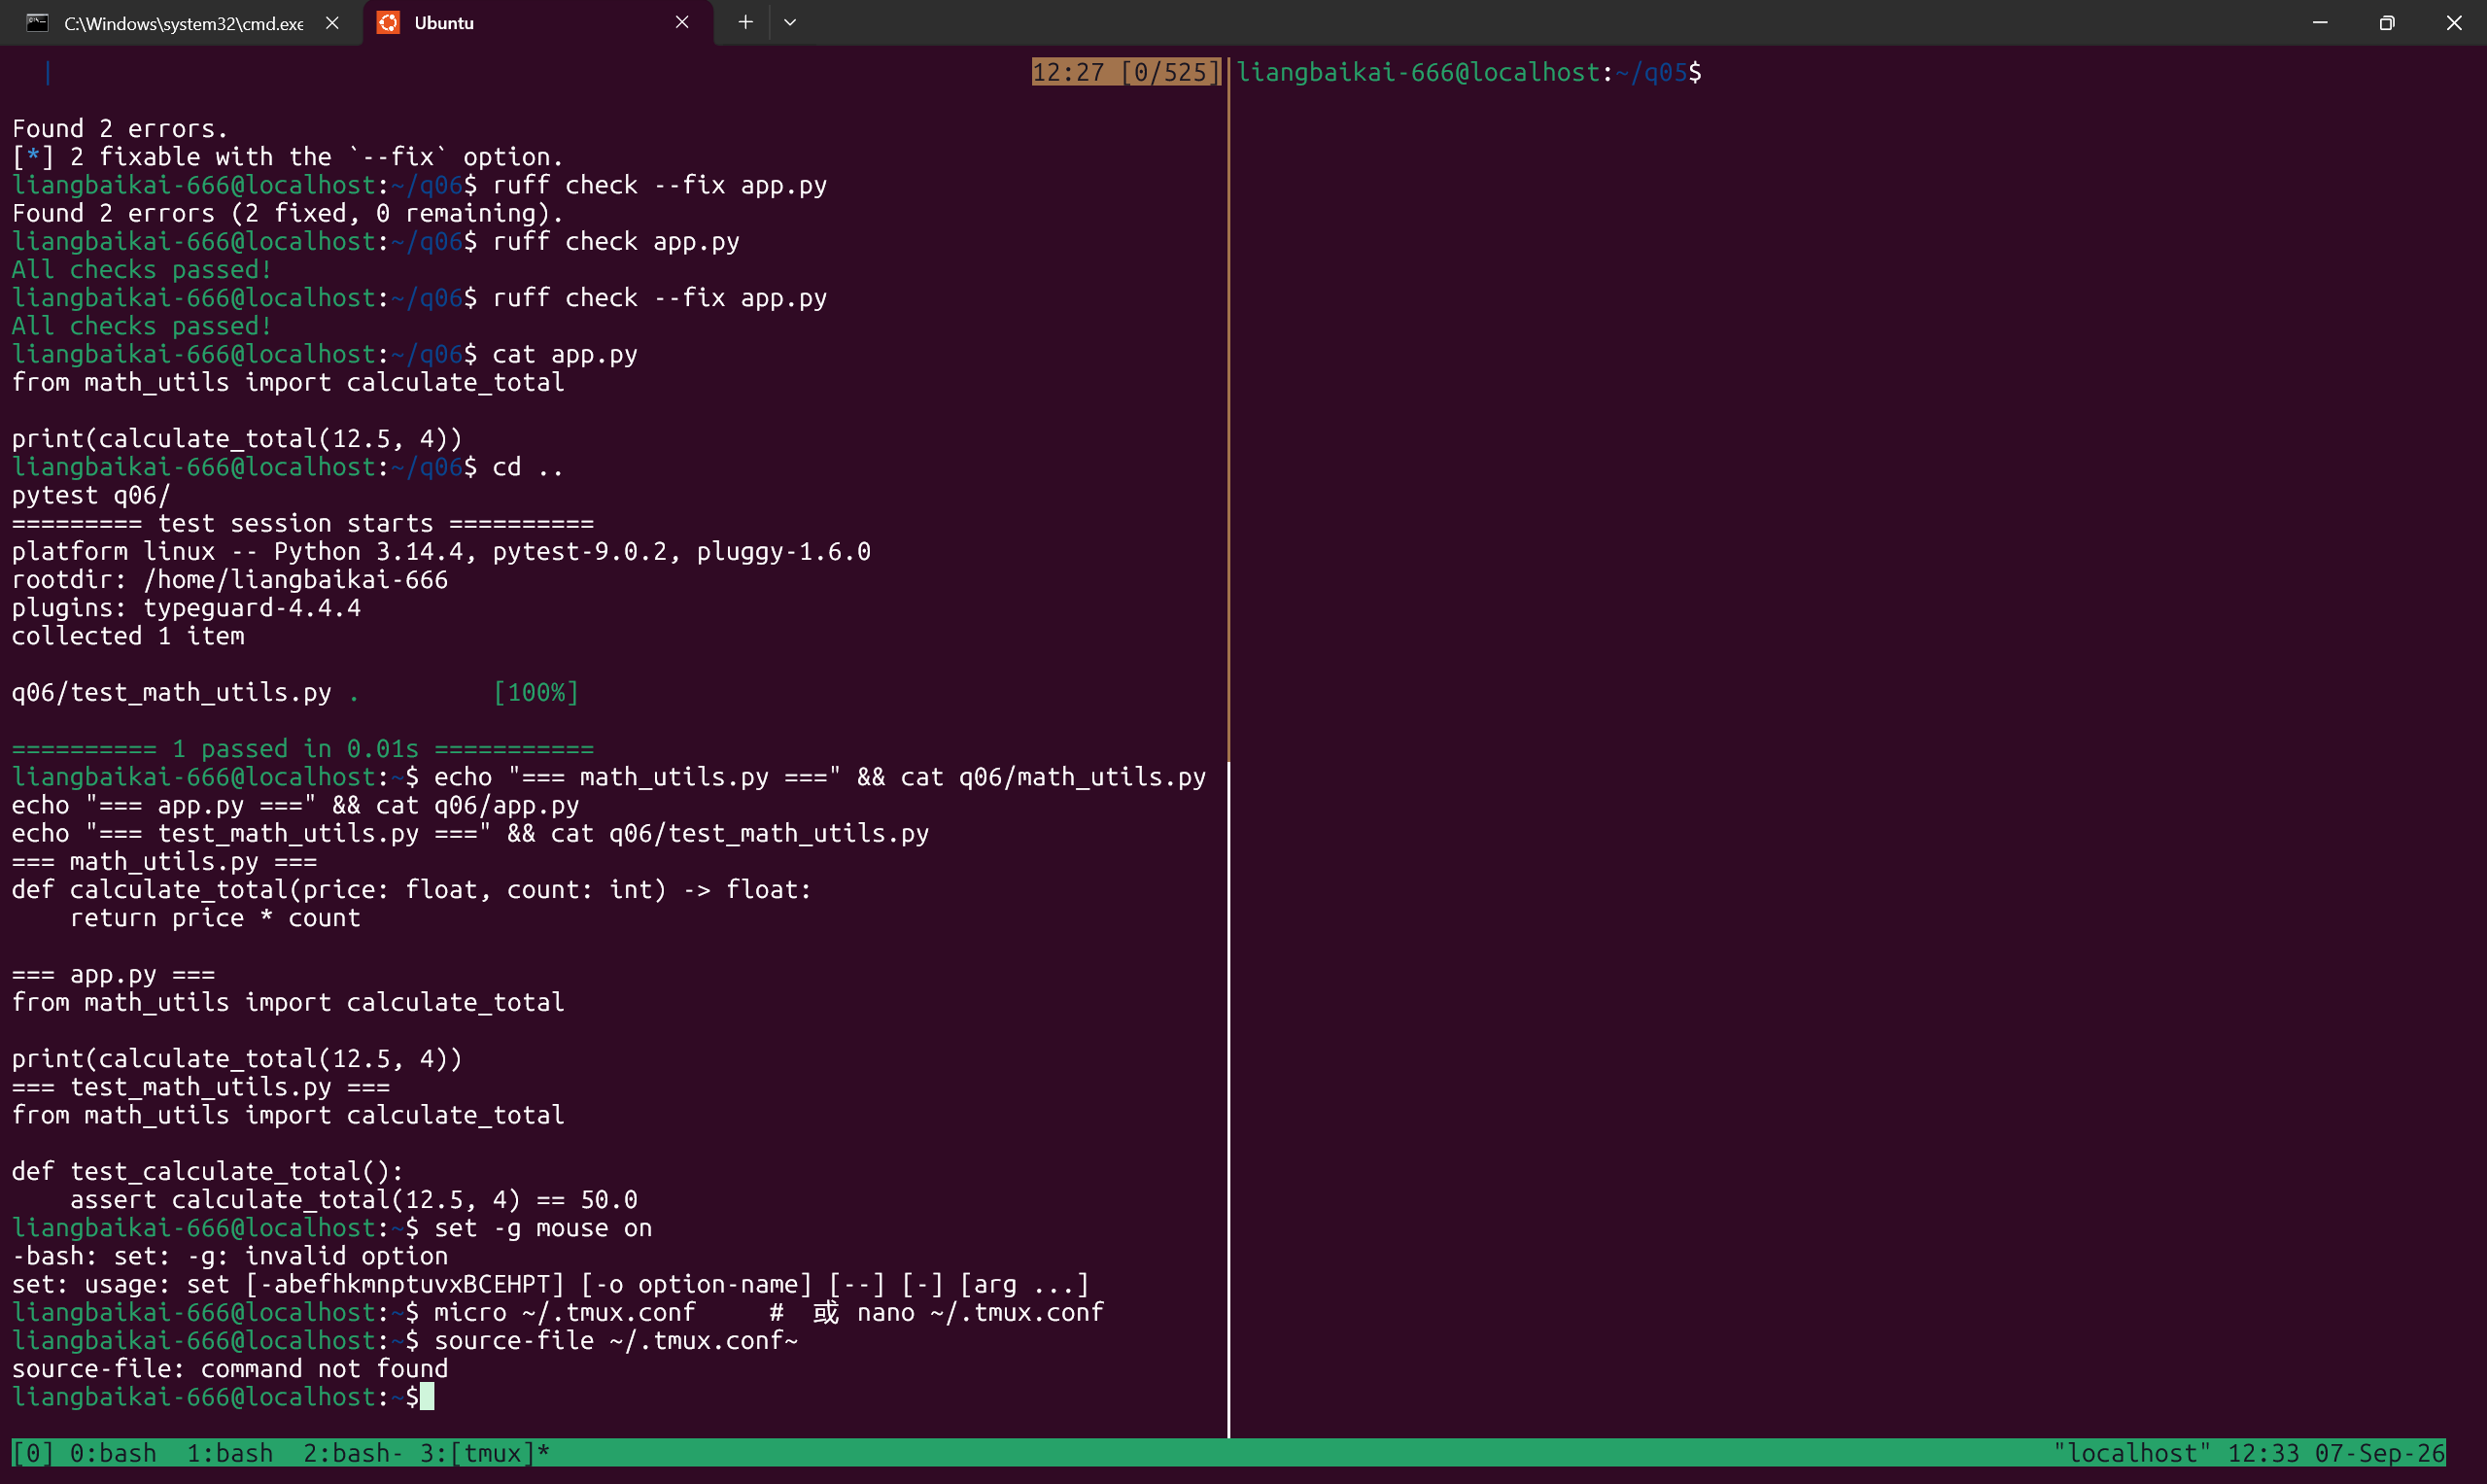
\includegraphics[width=\linewidth]{q06-3.png}
    \caption{\texttt{ruff check --fix} 自动修复后全部检查通过，\texttt{pytest} 测试通过}
  \end{subfigure}
  \caption{q06：重构、静态检查与单元测试}
  \label{fig:q06}
\end{figure}

\subsection{结果分析}

\begin{itemize}
  \item \textbf{查找引用}：\texttt{grep -rn "total\_price" *.py} 定位到全部
        6 处出现——\texttt{math\_utils.py:1}（定义）、\texttt{app.py:1--2}
        （导入与调用）、\texttt{test\_math\_utils.py:1/3/4}（导入、测试函数名、断言），
        等效于语言服务器的 Find References；
  \item \textbf{语义重命名同步性}：\texttt{sed} 批量替换后再次 \texttt{grep} 验证，
        定义与所有引用（含测试函数名 \texttt{test\_total\_price} →
        \texttt{test\_calculate\_total}）同步更新为 \texttt{calculate\_total}，
        无遗漏残留；与 IDE 中``重命名符号''的效果一致——后者基于语言服务器
        的作用域分析给出预览，本实验在终端以文本方式达成同样目标；
  \item \textbf{ruff 反馈环}：临时加入的 \texttt{import os} 被 ruff 以
        F401（未使用导入）报告，并伴随导入排序问题（Organize imports）；
        \texttt{ruff check --fix} 自动修复 2 处问题，复查输出
        \texttt{All checks passed!}，体现了``检查—自动修复—复查''的本地开发反馈闭环；
  \item \textbf{pytest 回归}：重命名后运行 \texttt{pytest}，
        测试函数因 \texttt{test\_} 前缀仍被自动收集，
        \texttt{1 passed in 0.01s}，确认重构未改变程序行为。
\end{itemize}

% ============================================================
\section{q07：用调试器定位归并排序缺陷}

\subsection{题目要求}

主题：Debugging。将存在缺陷的归并排序代码保存为 \texttt{q07/merge\_sort.py}，
再使用调试器定位并修复：
\begin{itemize}
  \item 先运行给定输入，确认结果错误或出现异常；
  \item 使用 pdb、IDE debugger 或等价调试器，在 \texttt{merge} 中设置断点并观察
        \texttt{i}、\texttt{j}、\texttt{left[i]}、\texttt{right[j]}；
  \item 完成最小修复，不得用 \texttt{sorted} 替换归并排序；
  \item 使用 pytest 增加两个测试：给定输入和含重复元素的列表；保证测试通过。
\end{itemize}

\subsection{实验步骤}

按题目给定内容写入缺陷代码：

\begin{lstlisting}[language=Python]
def merge(left, right):
    result = []
    i = j = 0
    while i < len(left) and j < len(right):
        if left[i] <= right[j]:
            result.append(left[i]); i += 1
        else:
            result.append(right[i]); j += 1  # 此处存在缺陷
    return result + left[i:] + right[j:]

def merge_sort(a):
    if len(a) <= 1: return a
    m = len(a) // 2
    return merge(merge_sort(a[:m]), merge_sort(a[m:]))

print(merge_sort([3, 1, 4, 1, 5, 9, 2, 6]))
\end{lstlisting}

运行确认错误，并用最小输入单独验证 \texttt{merge}：

\begin{lstlisting}[language=bash]
python3 merge_sort.py
# [1, 2, 4, 3, 4, 5, 6, 9]  ← 输出乱序且含重复, 确认结果错误

python3 -c 'from merge_sort import merge; print(merge([1, 3], [2, 4]))'
# [1, 4, 3, 4]  ← 最小输入即可复现: 问题定位在 merge
\end{lstlisting}

用 pdb 在 \texttt{merge} 处设断点，单步观察变量
（首次会话因表达式输入报错而中止，清理 \texttt{q07} 后重做，第二次会话完成）：

\begin{lstlisting}[language=bash]
python3 -m pdb merge_sort.py
(Pdb) b merge_sort.merge        # 在 merge 设断点 → Breakpoint 1
(Pdb) c                         # 运行至断点
(Pdb) n                         # 单步执行
(Pdb) p left, right             # 观察两个输入子序列
(Pdb) p i, j                    # 观察索引
(Pdb) p left[i], right[j]       # 观察待比较元素
(Pdb) p result                  # 观察已归并结果
(Pdb) q
\end{lstlisting}

观察到 \texttt{else} 分支取用的是 \texttt{right[i]} 而非 \texttt{right[j]}——
索引用错导致元素被跳过或重复写入。完成最小修复：

\begin{lstlisting}[language=Python]
# merge_sort.py  (仅改动一处)
result.append(right[j]); j += 1  # 修复: right[i] -> right[j]
\end{lstlisting}

修复后运行并新增两个 pytest 测试：

\begin{lstlisting}[language=Python]
# test_merge_sort.py
from merge_sort import merge_sort

def test_given_input():
    assert merge_sort([3, 1, 4, 1, 5, 9, 2, 6]) == [1, 1, 2, 3, 4, 5, 6, 9]

def test_with_duplicates():
    assert merge_sort([2, 2, 1, 1]) == [1, 1, 2, 2]
\end{lstlisting}

\begin{lstlisting}[language=bash]
python3 merge_sort.py          # [1, 1, 2, 3, 4, 5, 6, 9]  ← 输出正确
pytest -v
# test_merge_sort.py::test_given_input PASSED      [ 50%]
# test_merge_sort.py::test_with_duplicates PASSED  [100%]
# 2 passed in 0.00s
\end{lstlisting}

\subsection{运行结果与截图}

图~\ref{fig:q07} 展示了 pdb 断点调试、最小修复与测试通过的全过程。

\begin{figure}[htbp]
  \centering
  \begin{subfigure}[b]{0.98\textwidth}
    \centering
    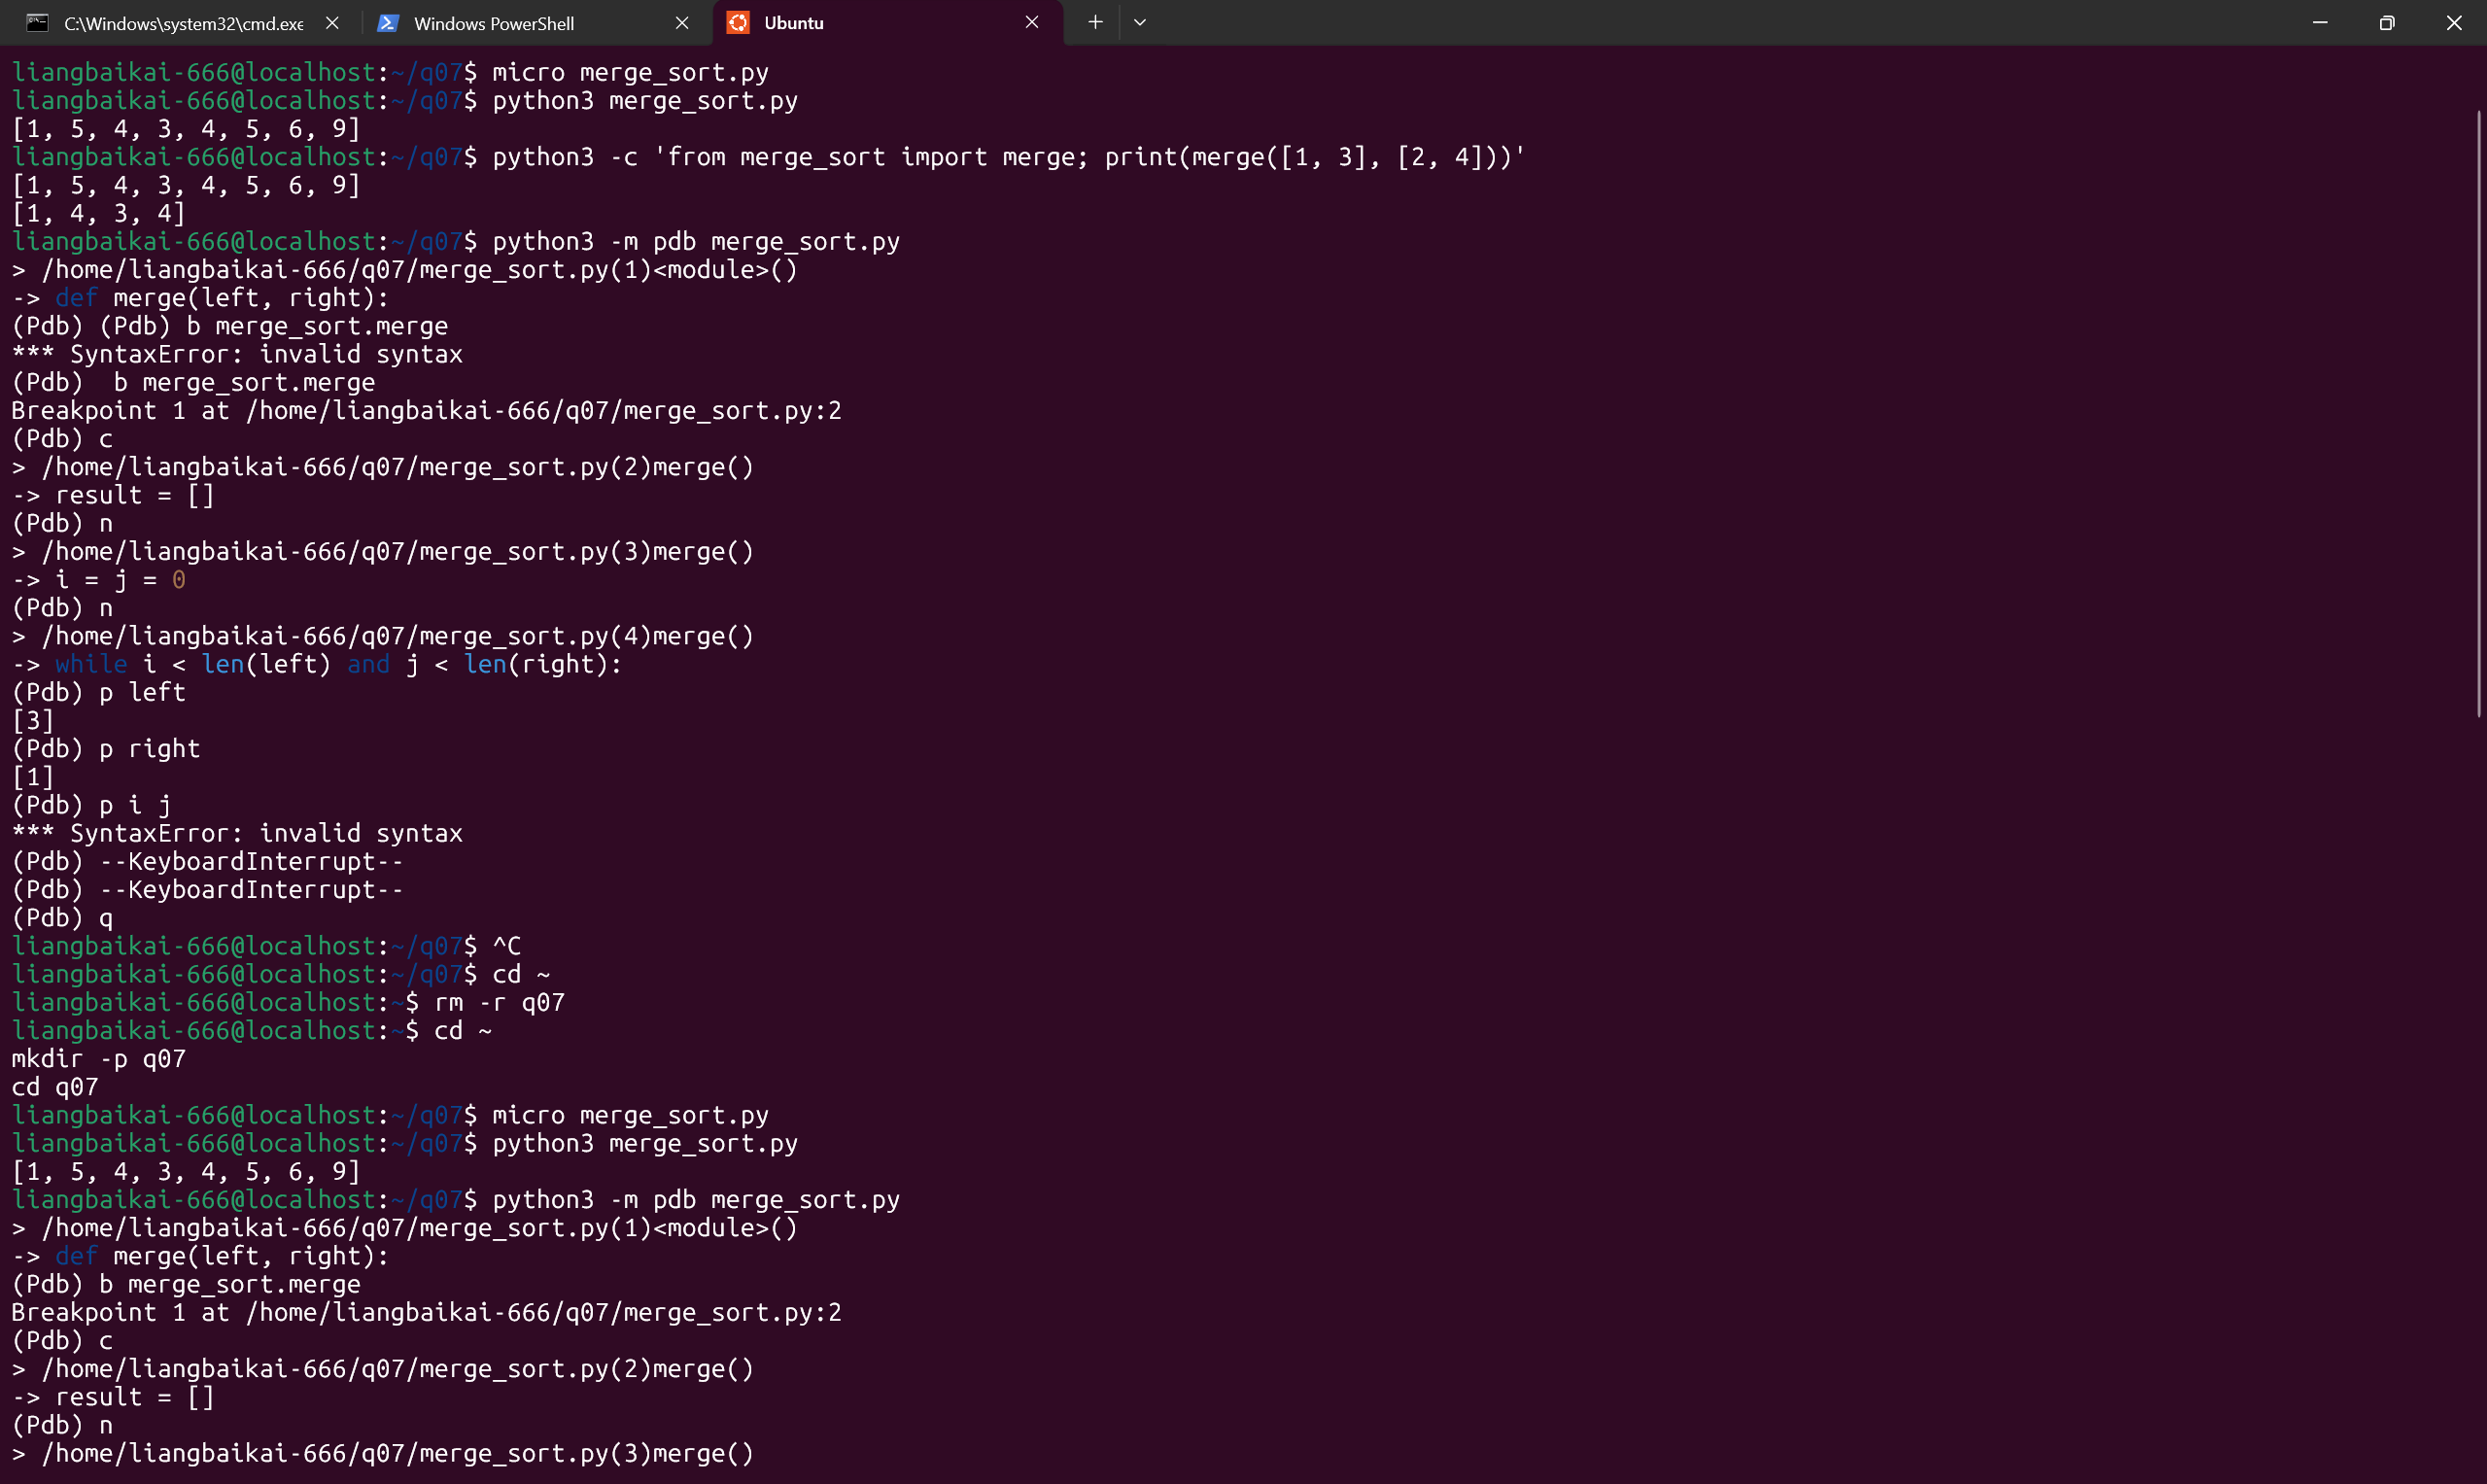
\includegraphics[width=\linewidth]{q07-1.png}
    \caption{编写 \texttt{merge\_sort.py}，\texttt{python3 -m pdb} 设断点单步调试（首次尝试后重做）}
  \end{subfigure}

  \vspace{0.5em}
  \begin{subfigure}[b]{0.98\textwidth}
    \centering
    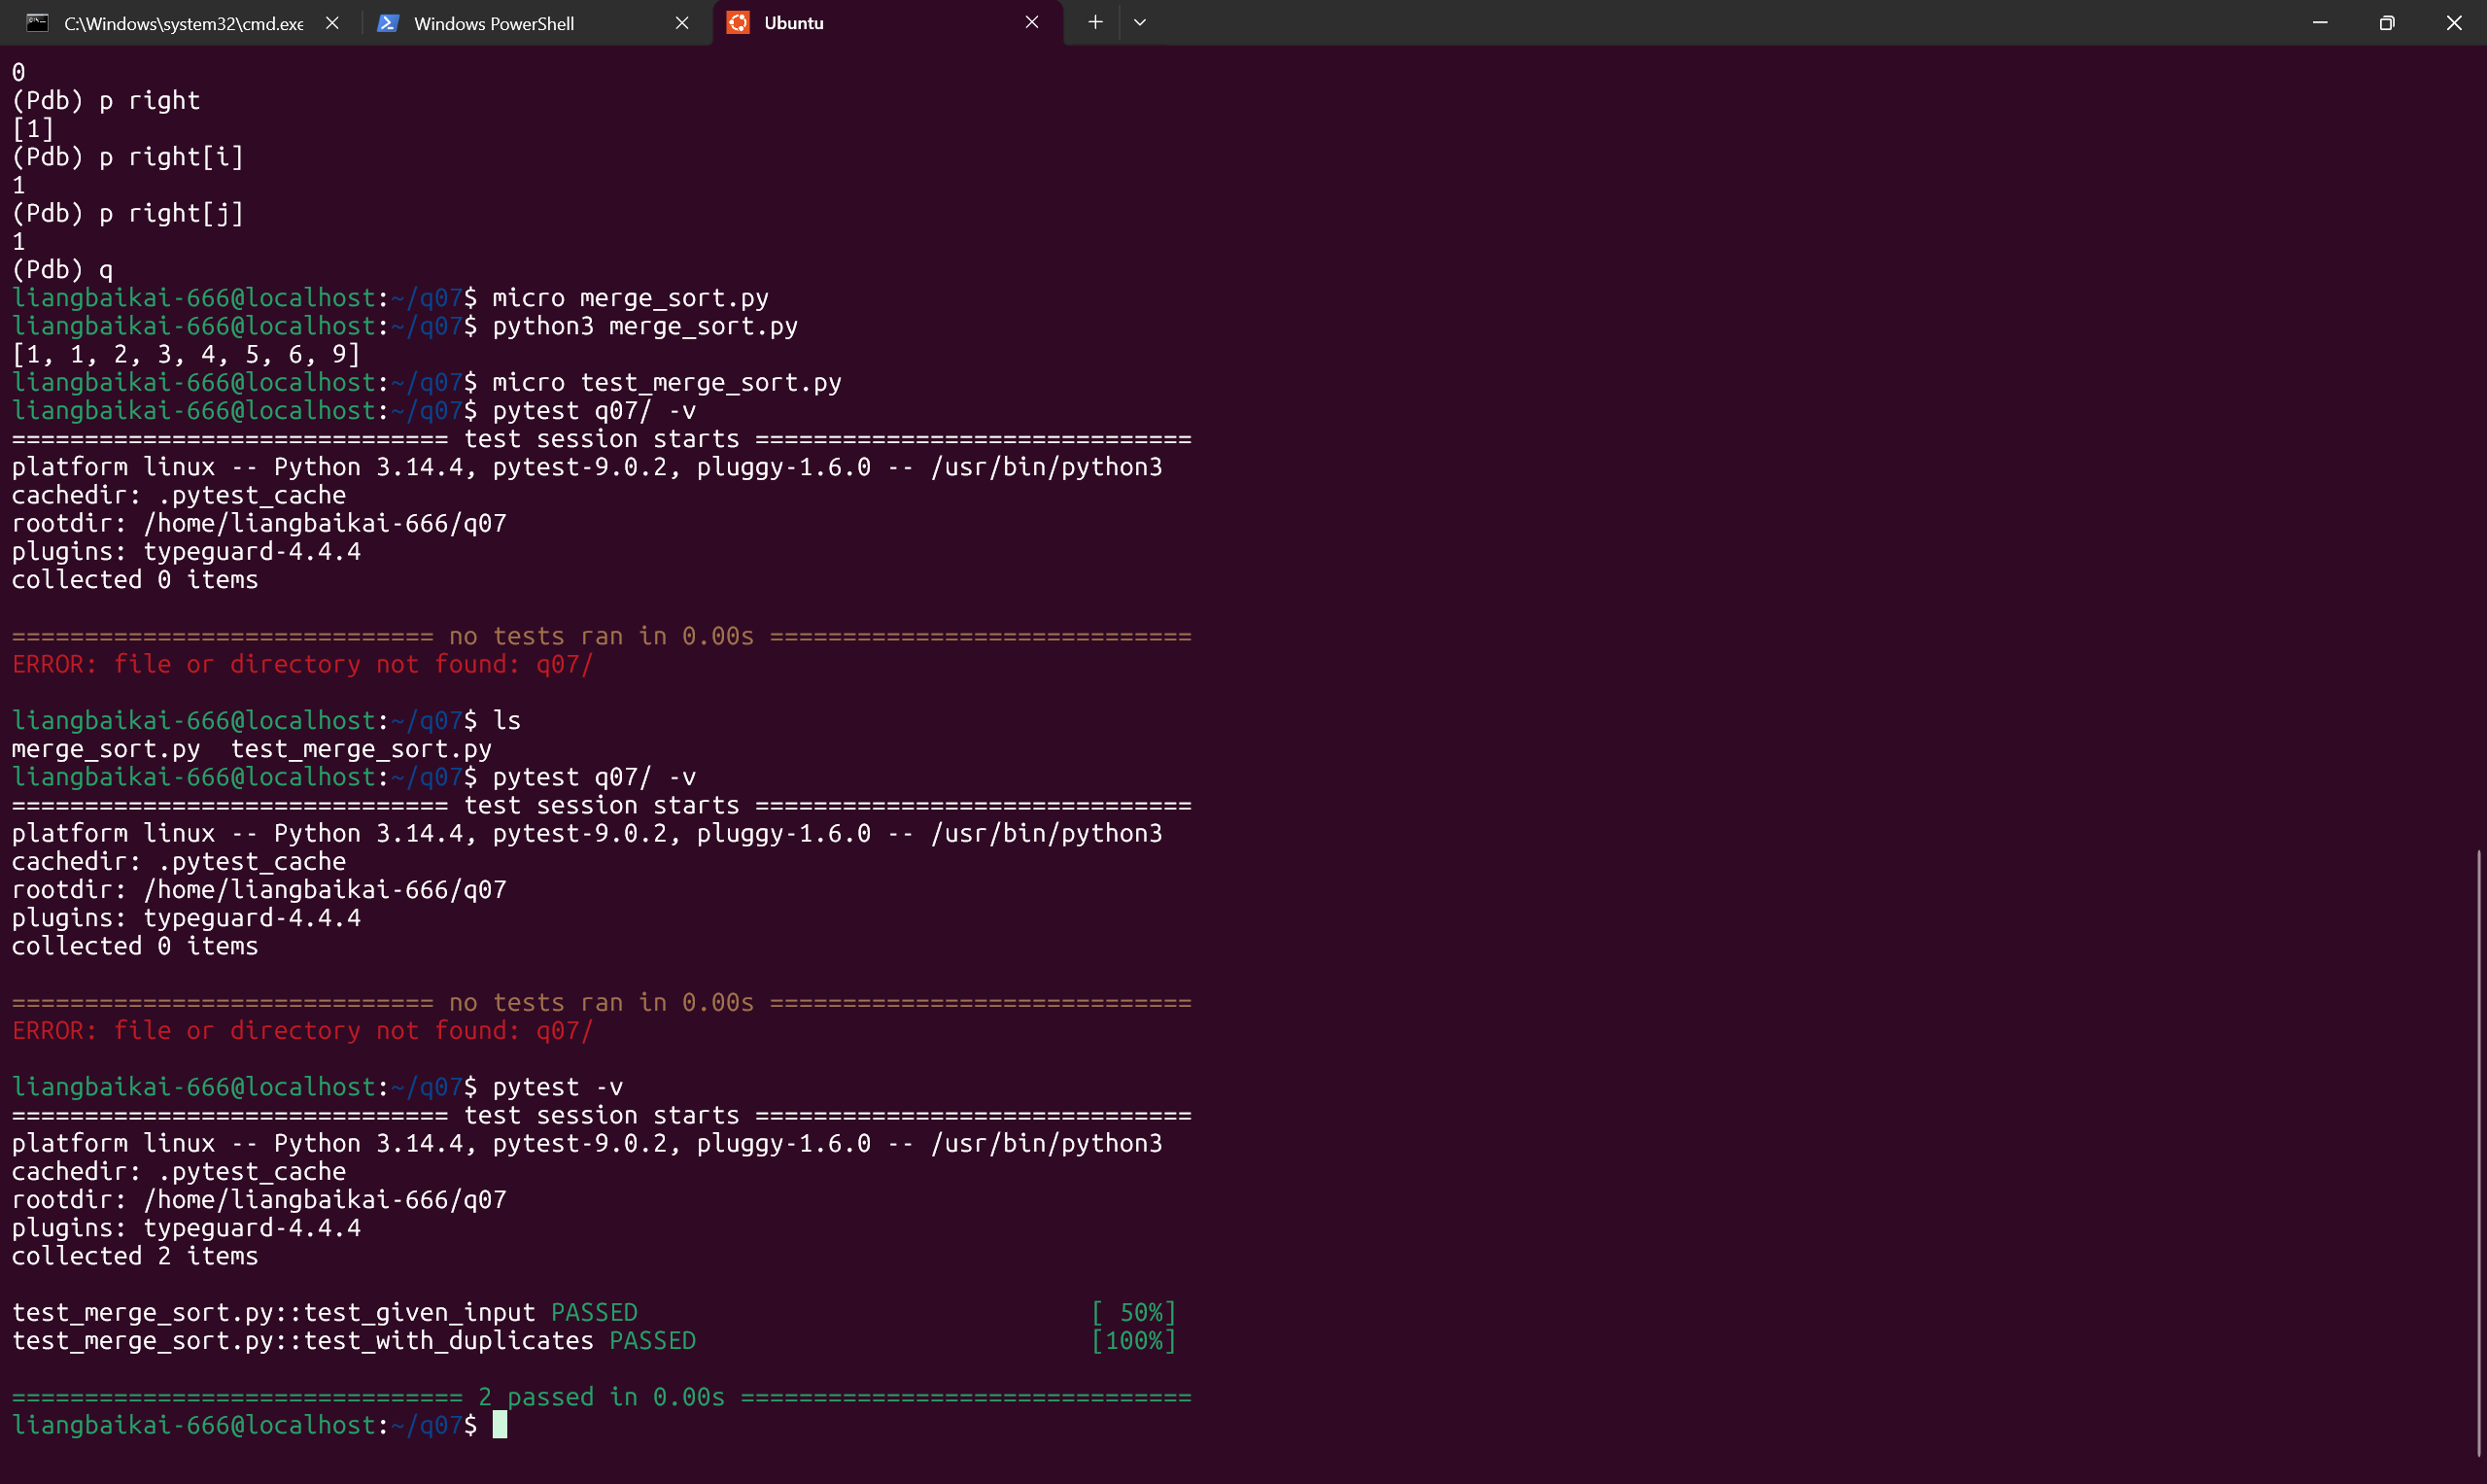
\includegraphics[width=\linewidth]{q07-2.png}
    \caption{pdb 检查变量后退出，排序输出 \texttt{[1, 1, 2, 3, 4, 5, 6, 9]}，\texttt{pytest -v} 2 项测试全部通过}
  \end{subfigure}
  \caption{q07：使用 pdb 调试归并排序}
  \label{fig:q07}
\end{figure}

\subsection{结果分析}

\begin{itemize}
  \item \textbf{缺陷确认}：运行给定输入输出 \texttt{[1, 2, 4, 3, 4, 5, 6, 9]}
        （正确应为 \texttt{[1, 1, 2, 3, 4, 5, 6, 9]}），乱序且元素错位；
        用最小输入 \texttt{merge([1, 3], [2, 4])} 复现得 \texttt{[1, 4, 3, 4]}，
        将问题范围缩小到 \texttt{merge} 函数本身；
  \item \textbf{调试器定位}：\texttt{pdb} 中 \texttt{b merge\_sort.merge} 设断点，
        \texttt{c}/\texttt{n} 单步推进，\texttt{p left, right}、\texttt{p i, j}、
        \texttt{p left[i], right[j]}、\texttt{p result} 逐项观察，
        发现 \texttt{else} 分支在 \texttt{j} 停滞的情况下取用
        \texttt{right[i]}——右序列索引用错，导致元素被跳过或重复追加；
  \item \textbf{最小修复}：仅改动一处 \texttt{right[i]} → \texttt{right[j]}，
        未使用 \texttt{sorted} 替换算法，符合题目要求；
  \item \textbf{测试回归}：新增 \texttt{test\_given\_input} 与
        \texttt{test\_with\_duplicates} 两项测试，\texttt{pytest -v} 输出
        \texttt{2 passed}，验证修复正确且对重复元素稳健；
  \item \textbf{调试备注}：首次 pdb 会话因在提示符下输入了非法表达式
        （\texttt{SyntaxError}）而中断，清理目录重做后完成；另外在
        \texttt{\textasciitilde/q07} 目录内误执行 \texttt{pytest q07/} 会报
        \texttt{file or directory not found}——pytest 的路径参数是相对当前目录的，
        换到正确目录运行后一切正常。
\end{itemize}

% ============================================================
\section{q08：先测量，再优化慢速词频程序}

\subsection{题目要求}

主题：Profiling。在 q08 中创建可重复生成的词表和故意低效的去重程序，
再使用性能分析工具优化：
\begin{itemize}
  \item 生成 \texttt{words.txt}，使用 \texttt{time} 运行原程序 2 次并记录耗时；
  \item 使用 \texttt{cProfile -s cumulative} 运行一次，找出主要耗时位置；
  \item 在不改变最终 count 的前提下优化程序；不得写死 1000；
  \item 使用相同输入再运行 2 次，计算优化前后中位数和加速比。
\end{itemize}

\subsection{实验步骤}

按题目给定内容创建两个文件（\texttt{generate\_words.py} 以固定种子保证数据可复现，
\texttt{wordfreq.py} 使用列表做去重、故意低效）：

\begin{lstlisting}[language=Python]
# generate_words.py
import random
random.seed(20260831)
vocab = [f"w{i}" for i in range(1000)]
with open("words.txt", "w", encoding="utf-8") as f:
    f.write(" ".join(random.choice(vocab) for _ in range(30000)))

# wordfreq.py (优化前)
words = open("words.txt", encoding="utf-8").read().split()
unique = []
for word in words:
    if word not in unique:      # list 成员测试 O(k)
        unique.append(word)
print("count=", len(unique))
\end{lstlisting}

生成数据、计时 2 次、cProfile 剖析：

\begin{lstlisting}[language=bash]
python3 generate_words.py
ls -lh words.txt                # 144K

time python3 wordfreq.py        # count= 1000  real 0m0.105s
time python3 wordfreq.py        # count= 1000  real 0m0.104s

python3 -m cProfile -s cumulative wordfreq.py
# 1012 function calls in 0.096 seconds
#   ncalls  tottime  percall  cumtime  filename:lineno(function)
#   1       0.094    0.094    0.096    wordfreq.py:1(<module>)
#   1000    0.000    0.000    0.000    {method 'append' of 'list' objects}
\end{lstlisting}

热点在模块级循环中的 \texttt{word not in unique}——列表成员测试为线性扫描。
将 \texttt{unique} 改为集合（最小改动，其余不变）：

\begin{lstlisting}[language=Python]
# wordfreq.py (优化后, 仅两处改动)
words = open("words.txt", encoding="utf-8").read().split()
unique = set()
for word in words:
    if word not in unique:      # set 成员测试 O(1)
        unique.add(word)
print("count=", len(unique))
\end{lstlisting}

验证 count 不变，并以相同输入再计时 2 次：

\begin{lstlisting}[language=bash]
python3 wordfreq.py             # count= 1000  ← 与优化前一致

time python3 wordfreq.py        # count= 1000  real 0m0.019s
time python3 wordfreq.py        # count= 1000  real 0m0.018s
\end{lstlisting}

\subsection{运行结果与截图}

图~\ref{fig:q08} 展示了数据生成、优化前后计时对比与 cProfile 剖析结果。

\begin{figure}[htbp]
  \centering
  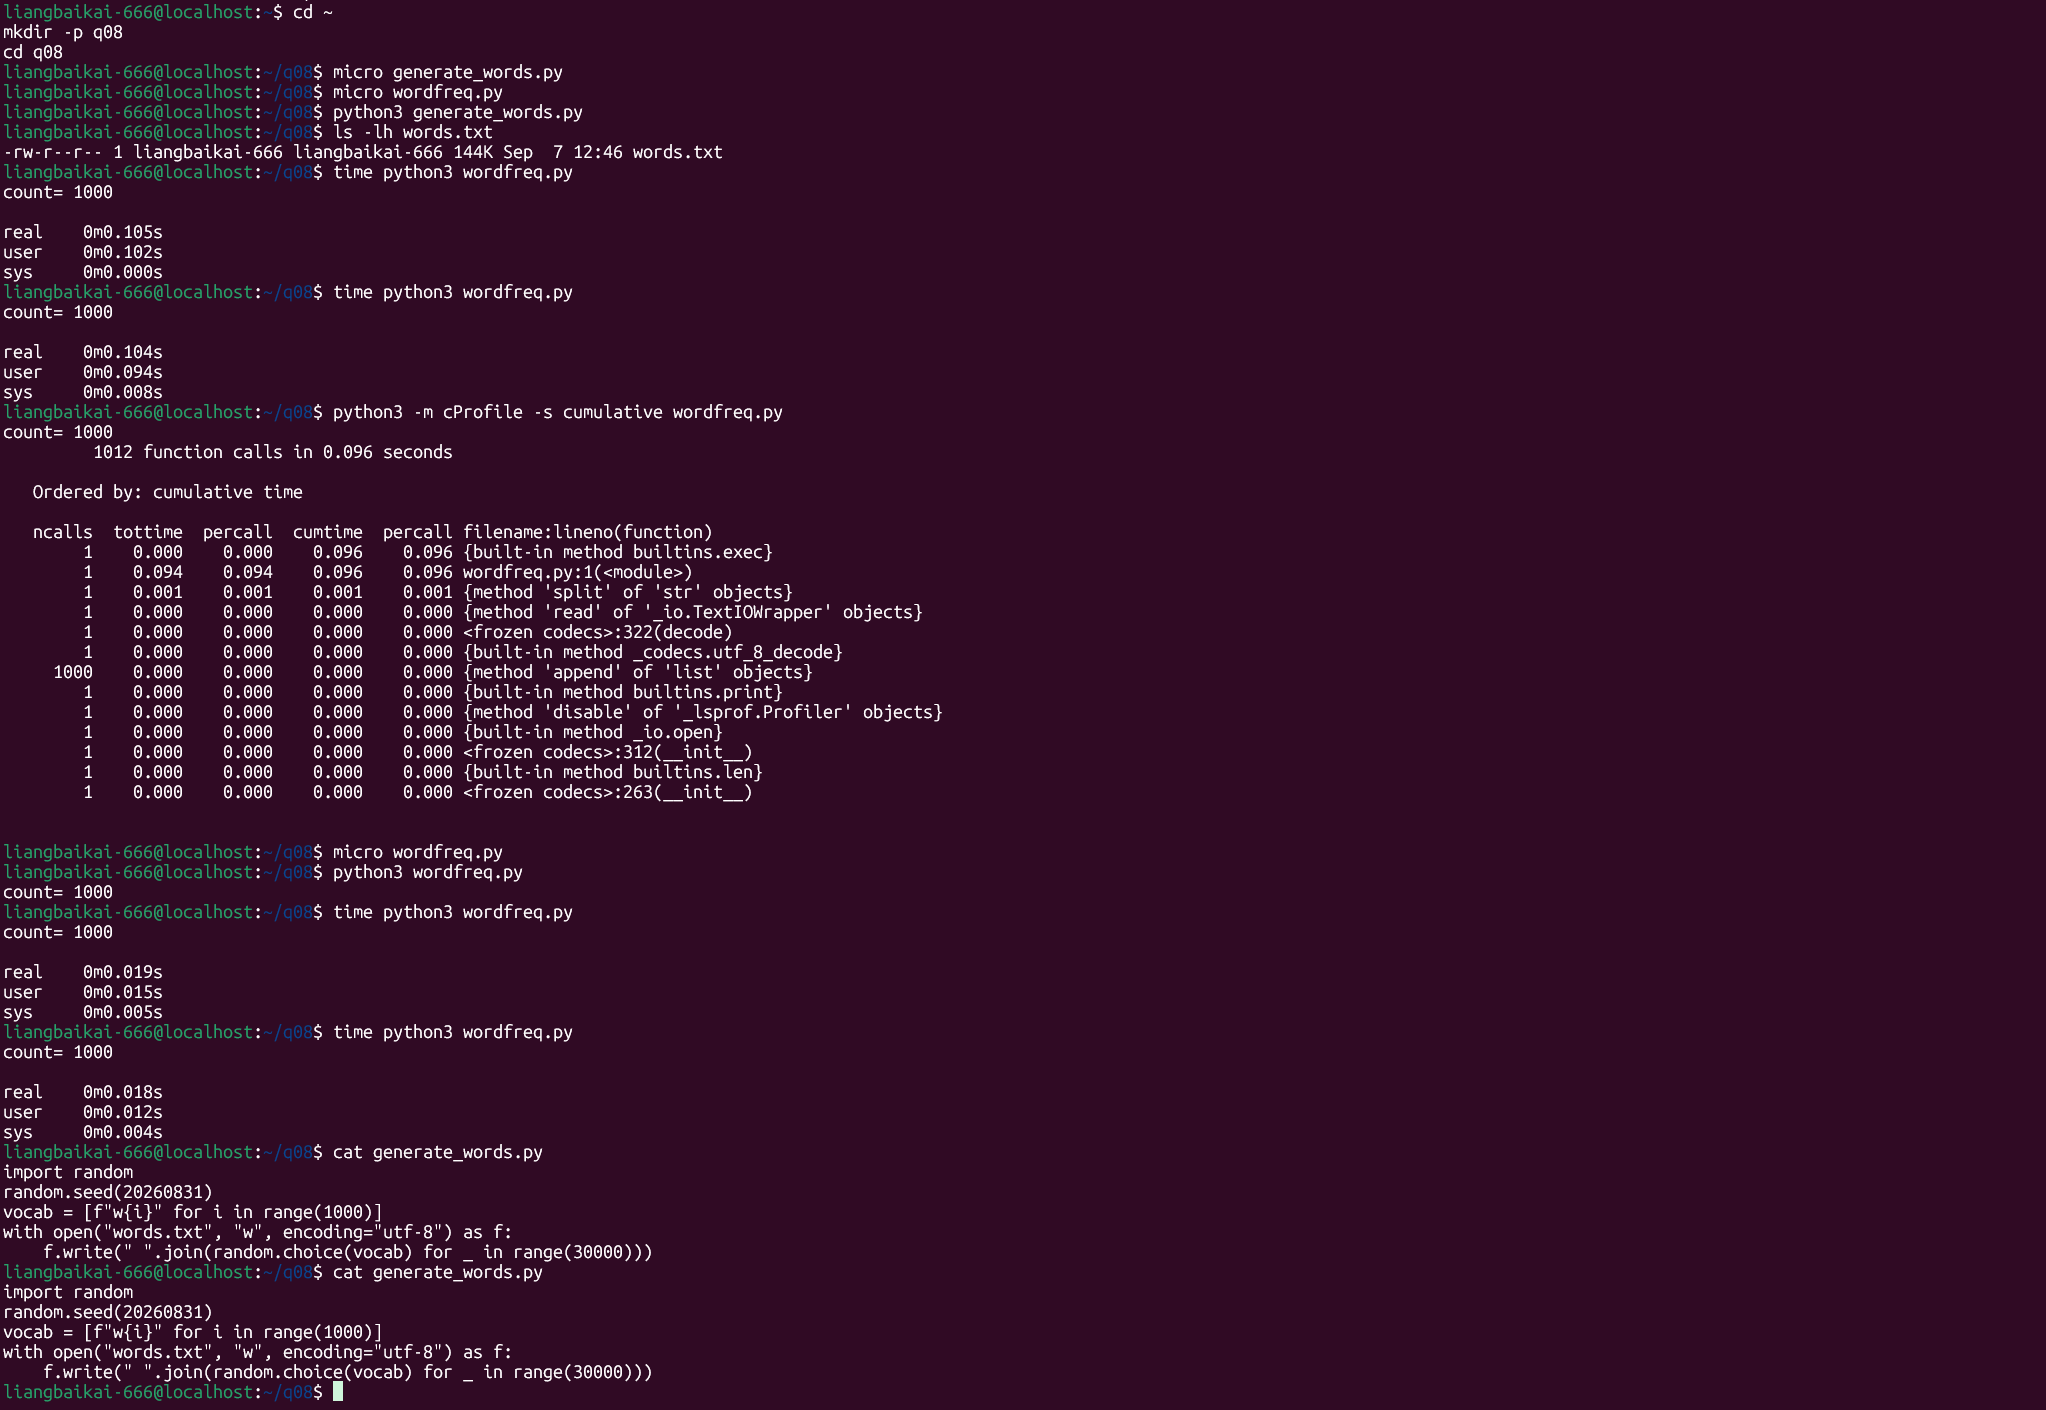
\includegraphics[width=0.98\textwidth]{q08-1.png}
  \caption{q08：生成测试数据，\texttt{time} 计时对比与 \texttt{cProfile} 剖析优化前后性能}
  \label{fig:q08}
\end{figure}

\subsection{结果分析}

\begin{itemize}
  \item \textbf{cProfile 定位热点}：\texttt{1012 function calls in 0.096 seconds}，
        累计时间几乎全部集中在 \texttt{wordfreq.py:1(<module>)}（\texttt{0.094s}）——
        即模块级的去重循环；\texttt{append} 恰好被调用 1000 次，
        印证 \texttt{unique} 最终增长到 1000 个元素，
        每次 \texttt{word not in unique} 都要对列表做线性扫描，
        总复杂度为 $O(n \cdot k)$（$n{=}30000$ 个词、$k{=}1000$ 个唯一词）；
  \item \textbf{优化方案}：将 \texttt{unique} 由 \texttt{list} 换成 \texttt{set}，
        哈希成员测试降为 $O(1)$，总复杂度降为 $O(n)$；
        count 由 \texttt{len()} 动态计算，未写死 1000，
        优化前后输出均为 \texttt{count= 1000}，语义不变；
  \item \textbf{中位数与加速比}：优化前两次耗时 \texttt{0.105s}/\texttt{0.104s}，
        中位数 \textbf{0.1045s}；优化后 \texttt{0.019s}/\texttt{0.018s}，
        中位数 \textbf{0.0185s}；加速比
        $0.1045 / 0.0185 \approx \mathbf{5.6}$ 倍；
  \item \textbf{可复现性}：\texttt{generate\_words.py} 使用固定种子
        \texttt{random.seed(20260831)}，\texttt{words.txt}（144K）内容确定，
        保证优化前后测量使用完全相同的输入，对比公平。
\end{itemize}

% ============================================================
\section{课后练习}

本节整理本周课后练习的解答，涵盖命令行基础、SSH 远程开发环境、
编辑器 Vim mode 配置以及调试与性能分析工具。

\subsection{命令行练习}

\subsubsection{1. \texorpdfstring{\texttt{-{}-}}{--} 的作用与文件操作}

\texttt{-{}-} 是``选项终止符''：它告诉命令解析器，后面的内容一律作为
普通参数（如文件名）处理，不再解析为选项或 flag。

\begin{lstlisting}[language=bash]
touch -- -myfile        # 创建名为 -myfile 的文件
rm ./-myfile            # 不使用 -- 时, 可加 ./ 路径前缀删除
\end{lstlisting}

\subsubsection{2. ls 常用参数组合}

\begin{lstlisting}[language=bash]
ls -lath --color=auto
\end{lstlisting}

\begin{table}[htbp]
  \centering
  \caption{ls 参数说明}\label{tab:lsargs}
  \begin{tabular}{ll}
    \toprule
    参数 & 含义 \\
    \midrule
    \texttt{-l} & 长格式显示 \\
    \texttt{-a} & 包含隐藏文件 \\
    \texttt{-h} & 易读大小（K/M/G） \\
    \texttt{-t} & 按修改时间排序 \\
    \texttt{-{}-color=auto} / \texttt{-G} & 输出带颜色 \\
    \bottomrule
  \end{tabular}
\end{table}

\subsubsection{3. 进程替换与 diff 比较环境变量}

\begin{lstlisting}[language=bash]
diff <(printenv | sort) <(export | sort)
\end{lstlisting}

两者输出不同的原因：
\begin{itemize}
  \item \textbf{格式不同}：\texttt{export} 输出带 \texttt{export } 前缀
        （如 \texttt{export KEY=value}），而 \texttt{printenv} 仅输出 \texttt{KEY=value}；
  \item \textbf{内容范围不同}：\texttt{export} 可能包含 Shell 函数等额外信息，
        而 \texttt{printenv} 只包含环境变量；
  \item \textbf{命令性质不同}：\texttt{export} 是 Shell 内建命令，
        \texttt{printenv} 是外部程序，两者获取信息的方式有差异。
\end{itemize}

\subsection{SSH 远程开发}

\begin{enumerate}
  \item \textbf{SSH 密钥}：检查 \texttt{ls \textasciitilde/.ssh/id\_ed25519*}；
        生成 \texttt{ssh-keygen -a 100 -t ed25519}；
  \item \textbf{SSH 配置}：在 \texttt{\textasciitilde/.ssh/config} 中写入题目所给的
        \texttt{Host vm} 配置；
  \item \textbf{复制公钥}：运行 \texttt{ssh-copy-id vm}；
  \item \textbf{端口转发验证}：虚拟机运行 \texttt{python -m http.server 8888}，
        本地浏览器访问 \texttt{http://localhost:9999} 能看到文件列表即成功；
  \item \textbf{SSH 服务安全加固}：编辑 \texttt{/etc/ssh/sshd\_config}，
        设置 \texttt{PasswordAuthentication no} 与 \texttt{PermitRootLogin no}，
        然后 \texttt{sudo service sshd restart}；
  \item \textbf{Mosh 挑战}：Mosh \textbf{能}正确恢复连接——它使用 UDP 并设计了
        连接恢复机制，短暂断网（如断开网卡）后网络恢复时可自动重连；
  \item \textbf{SSH 参数与后台转发}：\texttt{-N} 不执行远程命令，用于纯连接（如转发）；
        \texttt{-f} 后台运行 SSH 进程；后台端口转发可用
        \texttt{ssh -Nf vm}（利用 config 中的 LocalForward）或
        \texttt{ssh -Nf -L 9999:localhost:8888 user@host}。
\end{enumerate}

\subsection{Vim mode 与编辑器效率}

\subsubsection{在常用软件中启用 Vim mode}

\begin{itemize}
  \item \textbf{Bash}：\texttt{\textasciitilde/.bashrc} 加 \texttt{set -o vi}；
  \item \textbf{Zsh}：\texttt{\textasciitilde/.zshrc} 加 \texttt{bindkey -v}；
  \item \textbf{Fish}：\texttt{\textasciitilde/.config/fish/config.fish} 加
        \texttt{fish\_vi\_key\_bindings}；
  \item \textbf{Readline 程序}（Python REPL、irb 等）：\texttt{\textasciitilde/.inputrc} 加
        \texttt{set editing-mode vi}；
  \item \textbf{Git 提交/rebase 编辑器}：
        \texttt{git config --global core.editor "vim"}；
  \item \textbf{VS Code}：装 VSCodeVim，可选开启 \texttt{vim.useSystemClipboard}；
  \item \textbf{JetBrains}：装 IdeaVim；\textbf{Xcode}：Editor 菜单原生开启
        Vim Mode；\textbf{Qt Creator}：Preferences → FakeVim；
  \item \textbf{浏览器}：Chrome 装 Vimium，Firefox 装 Tridactyl。
\end{itemize}

\subsubsection{一个月只走 Vim mode}

日常写笔记、改配置、写代码全用普通模式优先：
\texttt{h j k l} 移动，\texttt{w b e} 跳词，
\texttt{ciw}、\texttt{ci"}、\texttt{di(} 改/删文本对象，
\texttt{yy}、\texttt{p}、\texttt{>}、\texttt{.}、\texttt{;} 复用上次操作。
觉得卡就搜``vim how to \ldots''，例如：
``move to next occurrence'' → \texttt{f\{char\}} / \texttt{t\{char\}} / \texttt{*}；
``edit in column'' → \texttt{Ctrl-v} 块选择；
``repeat complex edit'' → \texttt{qa ... q} 然后 \texttt{@a}。

\subsubsection{完成一道 VimGolf 并给项目配 IDE 扩展 + LSP}

\begin{lstlisting}[language=bash]
gem install vimgolf     # 安装
vimgolf setup           # 配置
vimgolf put <challenge_id>   # 完成一道挑战
\end{lstlisting}

以 VS Code 为例配置 IDE 扩展与 LSP：安装 VSCodeVim 与对应语言官方扩展
（Python / Rust / TypeScript / Go），确保语言服务器可用
（Python: \texttt{pylsp} 或 \texttt{basedpyright}；Rust: \texttt{rust-analyzer}；
Go: \texttt{gopls}）；打开项目中 import 的库符号，按 \texttt{gd} 或 \texttt{F12}
验证``跳转到定义''。

\subsection{调试与性能工具课程练习}

\begin{enumerate}
  \item \textbf{调试合并排序}：缺陷为 \texttt{merge} 的 \texttt{else} 分支
        误用索引 \texttt{i}（\texttt{right[i]}），修复为 \texttt{right[j]}——
        与正课 q07 相同；
  \item \textbf{rr 反向调试}：\texttt{curve\_scores} 循环条件 \texttt{i < 4}
        但 \texttt{scores} 数组仅 3 个元素（索引 0--2），\texttt{i = 3} 时
        数组越界写覆盖了相邻内存中的 \texttt{students[1].id}；
        用 \texttt{rr record ./corruption}、\texttt{rr replay} 配合
        \texttt{watch students[1].id} 与 \texttt{reverse-continue} 反向定位；
  \item \textbf{AddressSanitizer}：\texttt{uaf.c} 为释放后使用
        （Use-After-Free）——\texttt{free(greeting)} 后又执行
        \texttt{greeting[0] = 'J'}；ASan 报告 \texttt{heap-use-after-free}；
        修复为删除 free 之后的写操作，或在写之前重新分配内存；
  \item \textbf{strace}：\texttt{strace ls -l} 的主要系统调用包括
        \texttt{execve}（加载程序）、\texttt{openat}/\texttt{fstat}
        （读取目录与文件属性）、\texttt{write}（输出结果）、\texttt{close} 等；
  \item \textbf{LLM 辅助调试}：将编译器冗长报错（如 C++ 模板实例化失败、
        Rust 生命周期错误）或 ASan 完整输出交给 LLM，
        要求解释错误原因并给出修复代码；
  \item \textbf{perf stat}：\texttt{cycles}（CPU 时钟周期数）、
        \texttt{instructions}（指令总数）、\texttt{cache-misses}（缓存未命中次数）、
        \texttt{branch-misses}（分支预测失败次数）；
  \item \textbf{perf record 与火焰图}：\texttt{gcc -g -O2 slow.c -o slow -lm} 编译；
        \texttt{perf record -g ./slow} 采样；\texttt{perf report} 显示
        \texttt{slow\_computation} 占绝大部分时间；
        \texttt{perf script | stackcollapse-perf.pl | flamegraph.pl > flame.svg}
        生成交互式火焰图；
  \item \textbf{hyperfine 基准测试}：对比 \texttt{grep -R "pattern" .} 与
        \texttt{rg "pattern" .} 的耗时分布；
  \item \textbf{htop / taskset}：\texttt{taskset --cpu-list 0,2 stress -c 3}
        中 \texttt{-{}-cpu-list 0,2} 仅允许进程使用 CPU 0 与 CPU 2 两个核心，
        即使 \texttt{stress -c 3} 创建 3 个线程也无法利用第三颗 CPU；
  \item \textbf{端口占用排查}：\texttt{python -m http.server 4444} 启动服务；
        \texttt{ss -tlnp | grep 4444} 查找进程并记下 PID；\texttt{kill <PID>} 终止。
\end{enumerate}

% ============================================================
\section{代码与仓库}

项目已托管至 GitHub：
\url{https://github.com/liangbaikai-666/tool-25020007117}

\subsection{Git 提交记录}

% 待补充：commit log 文字版或截图（commit-log.png）

% ============================================================
\section{结论}

% 待补充：q06—q08 总结

\end{document}
